\section{Auswertung}
\label{sec:Auswertung}

\subsection{Bestimmung der Tiefe und der Größe der Fehlstellen mit einem A-Scan}
\label{subsec:A_scan_Fehlstellen}

Zur Bestimmung der Eindringtiefen müssen zunächst Laufzeitkorrekturen, die durch
die Schutzschichten auf den Sonden entstehen, berücksichtigt werden. Dafür wird der
mit der Schieblehre bestimmte Wert von der Höhe $h_{\symup{S}}=8{,}03\,$cm des Blocks
von dem des mit Ultraschall bestimmten Wertes $h_{\symup{US}}=8,07\,$cm subtrahiert.
Es muss also von allen Werten in dieser Messreihe die Differenz $\Delta h=0{,}04\,$cm
subtrahiert werden. In Tabelle \ref{tab:messwerte} sind die  bereits bereinigten
Messwerte zur Messung mit dem A-Scan, sowie die mit der Schieblehre bestimmten
Werte dargestellt. Zudem befinden sich dort die berechneten Werte für die Dicken
der Fehlstellen.

\begin{table}[htp]
	\begin{center}
    \caption{Messwerte zur Messung der Fehlstellen mit einem A-Scan und mit einer Schieblehre,
    sowie daraus berechnete Werte.}
    \label{tab:messwerte}
		\begin{tabular}{cccccccc}
		\toprule
			{Fehlstelle} & {$s_{\symup{1,A}}/$mm} & {$s_{\symup{2,A}}/$mm} & {$d_{\symup{A}}/$mm} &
      {$s_{\symup{1,S}}/$mm} & {$s_{\symup{2,S}}/$mm} & {$d_{\symup{S}}/$mm} & {$\Delta d$/mm}\\
			\midrule
			3   & 15,2 & 63,0 & 2,1 & 13,2 & 61,1 & 6,0 & 3,9\\
			4   & 23,7 & 55,8 & 0,8 & 21,6 & 53,7 & 5,0 & 4,2\\
			5   & 32,2 & 48,3 & -0,2 & 30,0 & 46,3 & 4,0 & 4,2\\
			6   & 41,0 & 41,1 & -1,8 & 38,6 & 38,7 & 3,0 & 4,8\\
			7   & 49,0 & 33,0 & -1,7 & 46,7 & 30,8 & 3,0 & 4,7\\
			8   & 56,7 & 24,8 & -1,2 & 54,7 & 22,8 & 3,0 & 4,2\\
			9   & 64,7 & 16,8 & -1,2 & 62,7 & 14,9 & 3,0 & 4,2\\
			10  & 73,3 & 8,8  & -1,8 & 70,6 & 6,9 & 3,0 & 4,8\\
			11  & 17,0 & 57,5 & 5,80 & 15,0 & 55,5 & 10,0 & 4,2\\
		\bottomrule
		\end{tabular}
	\end{center}
\end{table}

Dabei werden die Strecken, die in Abbildung \ref{fig:acrylblock} unterhalb der Fehlstellen liegen
als $s_1$ und die Strecken, die oberhalb der Fehlstellen liegen als $s_2$ bezeichnet.
Die Messwerte, die mit dem A-Scan aufgenommen wurden, werden mit dem Index "A"
und die, die mit der Schieblehre aufgenommen wurden mit dem Index "S" versehen.

Die Bestimmung der Dicke der Fehlstellen mithilfe des A-Scans erfolgt durch den
Zusammenhang
\begin{equation}
  d_{\symup{A}}=h_{\symup{S}}-s_{\symup{1,A}}-s_{\symup{2,A}} \,.
\end{equation}
Die Differenz $\Delta d$ der mit der Schieblehre und mit dem A-Scan bestimmten
Dicken ergibt sich durch
\begin{equation}
  \Delta d=|d_{\symup{A}}-d_{\symup{S}}| \,.
\end{equation}

Auffällig ist, dass diese Differenzen teilweise negativ sind und hohe Abweichungen
vom den mit der Schieblehre bestimmten Werten aufweisen.

In Tabelle \ref{tab:abweichunga} sind die relativen Abweichungen der durch den A-Scan
bestimmten Dicken von den mithilfe der Schieblehre bestimmten Dicken der Fehlstellen
dargestellt.

\begin{table}[htp]
	\begin{center}
		\caption{Relative Abweichungen der durch den A-Scan bestimmten Dicken der Fehlstellen
		von den mithilfe der Schieblehre bestimmten Dicken der Fehlstellen.}
		\label{tab:abweichunga}
		\begin{tabular}{cc}
		\toprule
			{Fehlstelle} & {$\Delta d/\%$}\\
			\midrule
			3 & -65\\
			4 & -84\\
			5 & -105\\
			6 & -160\\
			7 & -157\\
			8 & -140\\
			9 & -140\\
			10 & -160\\
			11 & -42\\
		\bottomrule
		\end{tabular}
	\end{center}
\end{table}

\subsection{Bestimmung des Auflösungsvermögens mit einem A-Scan}
\label{subsec:A_scan_auflösung}

Zur Bestimmung der Auflösung werden eine 1\,MHz-Sonde und eine 4\,MHz-Sonde verwendet
und die Fehlstellen 1 und 2 werden von beiden Seiten ausgemessen.
Die aufgenommenen Bilder für die Fehlstellen 1 und 2 befinden sich in den Abbildungen \ref{fig:auflösung1},
\ref{fig:auflösung2}, \ref{fig:auflösung3} und \ref{fig:auflösung4}.

\begin{figure}[H]
  \centering
  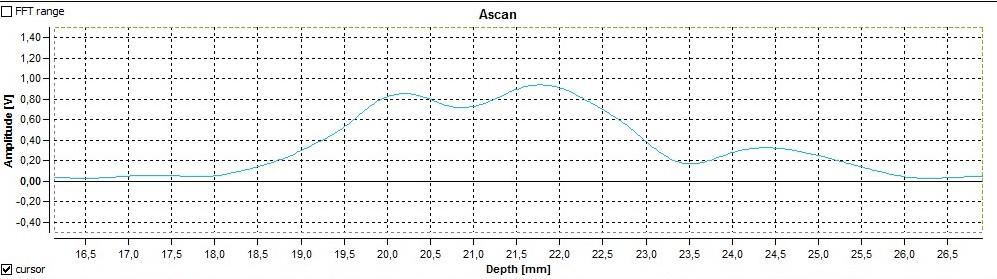
\includegraphics[width=\textwidth]{data/1mhzdoppelteFehlstellekurzelLaufzeitGedrehtwieinZeichnung.jpeg}
  \caption{Darstellung der Fehlstellen 1 und 2 mit einem A-Scan mit einer 1\,MHz-Sonde, wobei der Ultraschall
  zuvor die kurze Strecke durchlaufen musste.}
  \label{fig:auflösung1}
\end{figure}

\begin{figure}[H]
  \centering
  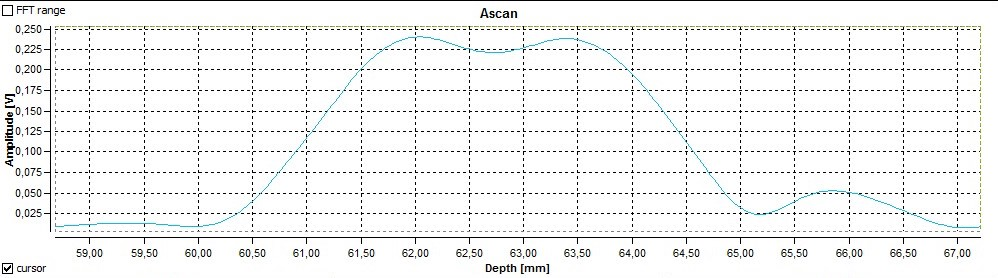
\includegraphics[width=\textwidth]{data/1mhzdoppelteFehlstellelangeLaufzeit.jpg}
  \caption{Darstellung der Fehlstellen 1 und 2 mit einem A-Scan mit einer 1\,MHz-Sonde, wobei der Ultraschall
  zuvor die lange Strecke durchlaufen musste.}
  \label{fig:auflösung2}
\end{figure}

\begin{figure}[H]
  \centering
  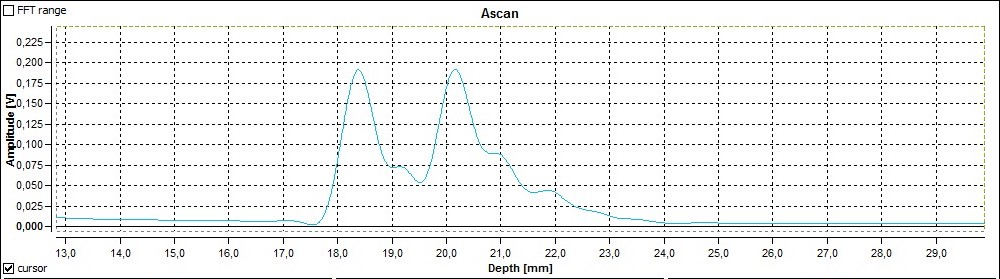
\includegraphics[width=\textwidth]{data/4mhzdoppelteFehlstellekurzelLaufzeitGedrehtwieinZeichnung.jpg}
  \caption{Darstellung der Fehlstellen 1 und 2 mit einem A-Scan mit einer 4\,MHz-Sonde, wobei der Ultraschall
  zuvor die kurze Strecke durchlaufen musste.}
  \label{fig:auflösung3}
\end{figure}

\begin{figure}[H]
  \centering
  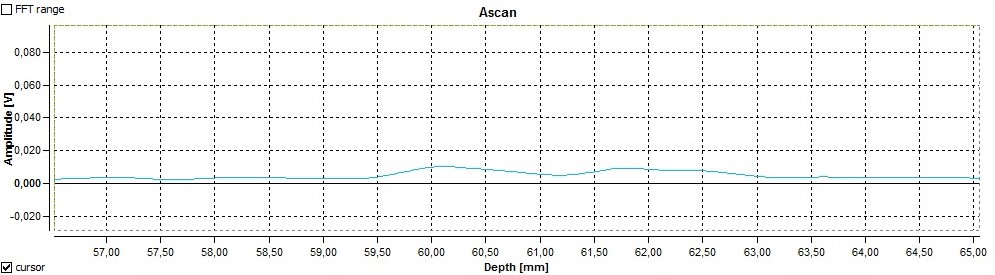
\includegraphics[width=\textwidth]{data/4mhzdoppelteFehlstellelangeLaufzeit.jpg}
  \caption{Darstellung der Fehlstellen 1 und 2 mit einem A-Scan mit einer 4\,MHz-Sonde, wobei der Ultraschall
  zuvor die lange Strecke durchlaufen musste.}
  \label{fig:auflösung4}
\end{figure}

Deutlich erkennbar ist, dass bei beiden Sonden die Amplitude bei einer längeren
Laufzeit abnimmt. Bei der Messung mit der 4\,MHz-Sonde tritt dieser Effekt jedoch
deutlich stärker auf und die Maxima sind kaum noch zu erkennen. Dafür liefert die
4\,MHz-Sonde jedoch bei einer kurzen Laufzeit ein deutlich schärferes Bild als die
1\,MHz-Sonde.

\subsection{Bestimmung der Tiefe und der Größe der Fehlstellen mit einem B-Scan}
\label{subsec:B_scan_Fehlstellen}

Zur Bestimmung der Lage und der Größe der Fehlstellen mit einem B-Scan muss zunächst
erneut die Laufzeitkorrektur durchgeführt werden. Der mithilfe des Ultraschalls bestimmte
Wert für die Höhe des Blocks beträgt $h=80{,}8\,$mm. Der Differenz zur mit der Schieblehre
bestimmten Wert beträgt also $\Delta h=0{,}5\,$mm. In Tabelle \ref{tab:b-scan}
sind die bereinigten Messwerte, sowie die daraus berechneten Werte dargestellt.
Für Fehlstelle 10 konnten dabei nicht alle Werte aufgenommen werden, da diese bei einer
Messung von Fehlstelle 11 überlagert wurde.

\begin{table}[htp]
	\begin{center}
    \caption{Messwerte zur Messung der Fehlstellen mit einem B-Scan und daraus berechnete Werte.}
    \label{tab:b-scan}
		\begin{tabular}{ccccc}
		\toprule
			{Fehlstelle} & {$s_{\symup{1,B}}/$mm} & {$s_{\symup{2,B}}/$mm} & {$d_{\symup{B}}/$mm} & {$\Delta d/$mm}\\
			\midrule
			3 & 12,8 & 61,1 & 6,4 & 0,4\\
			4 & 21,1 & 55,8 & 3,4 & 1,6\\
			5 & 29,7 & 48,3 & 2,3 & 1,7\\
			6 & 38,5 & 40,2 & 1,6 & 1,4\\
			7 & 46,5 & 31,9 & 1,9 & 1,1\\
			8 & 54,8 & 23,7 & 1,8 & 1,2\\
			9 & 62,6 & 15,4 & 2,3 & 0,7\\
			10 & {-} & 6,6 & {-} & {-} \\
		11 & 14,6 & 57,3 & 8,4 & 1,60\\
		\bottomrule
		\end{tabular}
	\end{center}
\end{table}

Die Rechnung erfolgt dabei analog zu der in Kapitel \ref{subsec:A_scan_Fehlstellen}.
In Tabelle \ref{tab:abweichungb} sind die relativen Abweichungen der mithilfe des B-Scans
bestimmten Dicken von den mithilfe der Schieblehre bestimmten Dicken der Fehlstellen
dargestellt.

\begin{table}[htp]
	\begin{center}
		\caption{Relative Abweichungen der mithilfe des B-Scans bestimmten Dicken der Fehlstellen
		von den mithilfe der Schieblehre bestimmten Dicken.}
		\label{tab:abweichungb}
		\begin{tabular}{cc}
		\toprule
			{Fehlstelle} & {$\Delta d/\%$}\\
			\midrule
			3 & 7\\
			4 & -32\\
			5 & -43\\
			6 & -47\\
			7 & -37\\
			8 & -40\\
			9 & -23\\
			10 & {-}\\
			11 & -16\\
		\bottomrule
		\end{tabular}
	\end{center}
\end{table}

In Abbildung \ref{fig:b-scan} ist beispielhaft für einen B-Scan der B-Scan des
Acrylblocks von der oberen Kante aus dargestellt.
\begin{figure}[H]
  \centering
  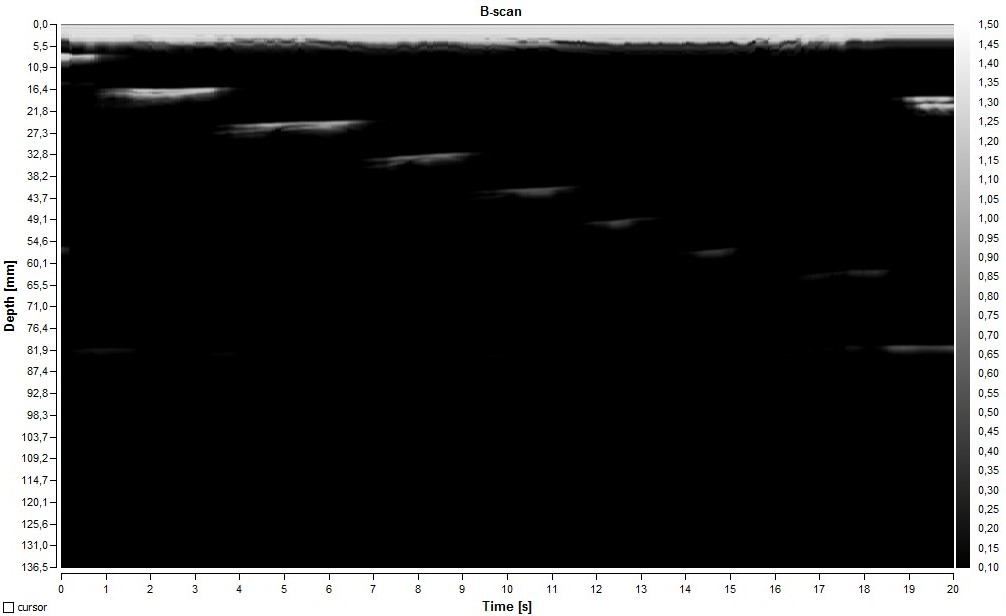
\includegraphics[width=15cm]{data/Bscanrechtsnachlinkswieinzeichnung.jpg}
  \caption{B-Scan des Acrylblocks von der oberen Kante aus.}
  \label{fig:b-scan}
\end{figure}

\newpage
\subsection{Bestimmung des Herzvolumens mit einem TM-Scan}
\label{subsec:Herzvolumen}


In Abbildung \ref{fig:herzvolumen} ist das im Versuch erstellte Diagramm der
simulierten Herschläge in Abhängigkeit von der Zeit dargestellt.

\begin{figure}[H]
  \centering
  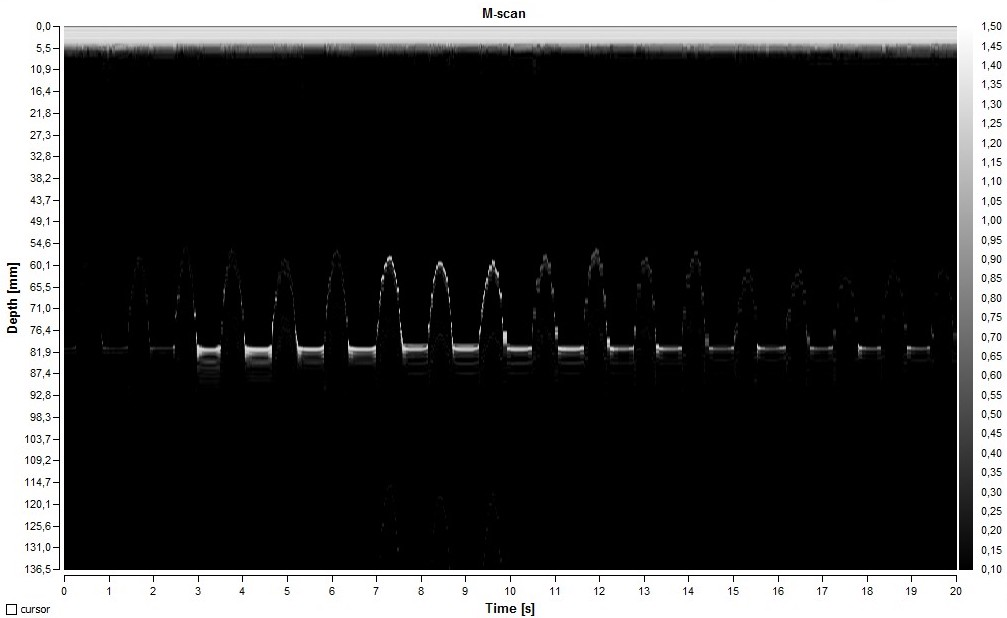
\includegraphics[width=15cm]{data/Herzfrequenz.jpg}
  \caption{Abhängigkeit der simulierten Herzschläge in Abhängigkeit von der Zeit; aufgenommen
  mit einem TM-Scan.}
  \label{fig:herzvolumen}
\end{figure}

Aus diesem Diagramm werden die Amplituden $s$ der Herzschläge abgelesen. Dabei
ist zu beachten, dass während der Messung noch ein falscher Wert für die Schallgeschwindigkeit
eingetragen war. Deshalb müssen alle abgelesenen Werte mit dem Quotienten
$\frac{c_{\symup{W}}}{c_{\symup{A}}}$ der Schallgeschwindigkeiten von Wasser
und Acryl multipliziert werden.

Das Luftvolumen, von dem das Wasser verdrängt wird, wird als Kugelsegment angenähert.
Es gilt damit für das Volumen
\begin{equation}
  V_s = \frac{h\pi}{6}\cdot(3r^2 + h^2) \,,
\end{equation}
wobei $r$ der Radius des verwendeten Zylinders und $h=s_0-s$ ist. Dabei ist $s$
die gemessene Eindringtiefe beim Herzschlag und $s_0$ die gemessene Strecke in
der Ausgangslage.

In Tabelle \ref{tab:herz} sind die aus dem Diagramm abgelesenen und bereits mit dem
Korrekturfaktor multiplizierten Werte, sowie daraus berechnete Werte zu sehen. Für den
ersten Schlag wird kein Wert abgelesen, da dieser nur sehr schlecht erkennbar ist.

\begin{table}[h!]
	\begin{center}
    \caption{Aus dem Diagramm abgelesene und mit dem Korrekturfaktor multiplizierte Werte und
    daraus berechnete Werte für die Höhe $h$ und das Volumen $V$ des Kugelsegments.}
    \label{tab:herz}
		\begin{tabular}{ccc}
		\toprule
			{$s/$mm} & {$h/$mm} & {$V/\symup{cm^3}$}\\
			\midrule
			31,3 & 12,8 & 11,9\\
			30,0 & 14,1 & 13,4\\
			30,1 & 14,0 & 13,3\\
			31,6 & 12,5 & 11,6\\
			30,1 & 14,0 & 13,3\\
			31,3 & 12,8 & 11,9\\
			31,6 & 12,5 & 11,6\\
			31,5 & 12,6 & 11,7\\
			31,1 & 13,0 & 12,2\\
			29,9 & 14,2 & 13,5\\
			31,9 & 12,2 & 11,3\\
			30,5 & 13,6 & 12,8\\
			32,9 & 11,2 & 10,2\\
			32,8 & 11,3 & 10,3\\
			34,5 & 9,6 & 8,5\\
			34,3 & 9,8 & 8,8\\
			34,1 & 10,0 & 9,0\\
		\bottomrule
		\end{tabular}
	\end{center}
\end{table}

Nach den Gleichungen
\begin{equation}
  \overline{x} = \frac{1}{N} \sum\limits_{i = 1}^N x_i
  \label{eqn:mean}
\end{equation}
und
\begin{equation}
  \sigma_x = \sqrt{\frac{1}{N(N-1)}
    \sum\limits_{i = 1}^N
    (x_i-\overline{x})^2}
    \label{eqn:std}
\end{equation}
wird der Mittelwert der Volumina $V$ zu $V_{\symup{mittel}}=11{,}5\pm1{,}6\,\symup{cm^3}$
berechnet.

Die Frequenz des simulierten Herzschlags ist $f=1{,}125\,$Hz. Damit ergibt sich
das gesuchte Herzvolumen\footnote{Es sei explizit darauf hingewiesen, dass dies kein
physikalisches Volumen darstellt und stattdessen eher einen Volumenstrom darstellt.} gemäß der Gleichung
\begin{equation}
  V_{\symup{Herz}} = V_{\symup{mittel}} f
\end{equation}
zu $V_{\symup{Herz}}=12{,}9\pm1{,}8\, \symup{\frac{cm^3}{s}}$.
